\section{Homepage}\label{homepage}
L'homepage rappresenta la vetrina del sito, è quindi necessario che convinca il visitatore a restare e a navigare all'interno del sito. Per fare ciò è importante che soddisfi le cosi dette ''6W''.

\subsection{Where?}
\begin{center}
\textit{A che tipo di sito sono arrivato?}
\end{center}

Questa informazione è facilmente intuibile, già dal nome del sito è possibile capire l'argomento principale del sito: \textit{la fotografia}.\\
Continuando poi a scorrere la pagina è possibile trovare la lista degli ultimi articoli scritti che è in grado di togliere ogni dubbio al visitatore riguardo l'argomento del sito.

\subsection{Who?}

\begin{center}
\textit{Chi rappresenta il sito?}
\end{center}

In alto a sinistra è presente il logo del sito, tuttavia questo non fornisce molte informazioni riguardo a chi gestisce il sito ed un click sul logo porta al refresh della homepage.\\
Per trovare maggiori informazioni riguardo a chi gestisce il sito è necessario scrollare fino al footer oppure selezionare nella navbar la voce \textit{Contatti > Chi c'è dietro FotoComeFare}.

\subsection{Why?}
\begin{center}
\textit{Quali benefici porta il sito?}
\end{center}

Il motivo per cui il visitatore dovrebbe restare nel sito è chiarito dal box rosso presente sulla destra della homepage. \\
Questo box descrive chiaramente le offerte del sito e fornisce anche la possibilità di iscriversi alla pagina di Facebook, specificando anche: ''\textit{Non spammeremo mai, potrai sempre disiscriverti}'' in modo da tranquillizzare l'utente.\\
Tuttavia è presente un grande problema riguardo questo box: la scelta dei colori, infatti, i colori scelti per il box sono troppo accessi e lo fanno sembrare un banner pubblicitario, creando il rischio che il visitatore lo ignori convinto che sia della pubblicità.

\begin{figure}[htpb]
\begin{center}
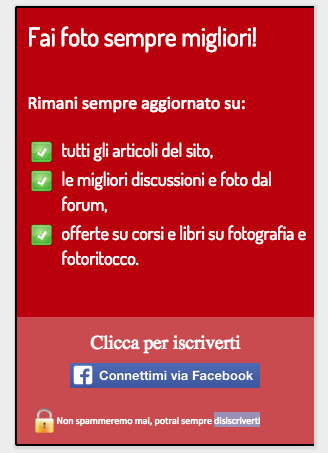
\includegraphics[width=0.5\textwidth]{immagini/boxRosso.png}
\caption{Box rosso presente nella homepage, la scelta dei colori lo fa sembrare un banner pubblicitario}
\label{boxRosso}
\end{center}
\end{figure}
\FloatBarrier

\subsection{What?}
\begin{center}
\textit{Che cosa offre il sito?}
\end{center}

Le ultime informazioni offerte dal sito sono subito presenti nella homepage. Vengono infatti, mostrati gli ultimi articoli secondo una visualizzazione a griglia, questa visualizzazione risulta ordinata e facilmente consultabile.\\
Inoltre, ogni articolo presente è dotato di un \textit{blurb} che fornisce una breve descrizione dell'articolo. 

\subsection{When?}
\begin{center}
\textit{Quanto è stato aggiornato il sito per l'ultima volta?}
\end{center}

Risulta facilmente intuibile che gli articoli presenti nella hompage siano disposti in ordine cronologico inverso, tuttavia non è presente alcuna data che fornisca all'utente un dato preciso riguardo l'ultimo aggiornamento.\\
Basterebbe aggiungere la data ad ogni articolo, in questo modo il visitatore riesce a farsi un'idea di ogni quanto viene aggiornato il sito e se alla prossima visita troverà dei contenuti nuovi.

\subsection{How?}
\begin{center}
\textit{Come faccio ad arrivare alle sezioni principali?}
\end{center}

La barra di navigazione presente nella parte alta del sito fornisce all'utente tutte le informazioni necessarie riguardanti il come muoversi sul sito, sono infatti presenti i vari link alle sezioni principali e la funzionalità di ricerca, quest'ultima rappresentata da una lente d'ingrandimento.\\
Nonostante sia usata una metafora visiva per la ricerca, questa è facilmente deducibile da parte del visitatore dato che l'icona delle lente d'ingrandimento è da molto tempo associata alla ricerca.

\subsection{Altre osservazioni}
Sempre in questa pagina è presente un ''carosello'' che mostra alcuni articoli di rilievo e che vengono alternati tra loro in modo automatico. Questa animazione potrebbe causare un po' di confusione agli utenti del sito che visualizzano la pagina per la prima volta.
